\section{反函数与复合函数}
\begin{definition}
设函数\(f\colon D \to f(D)\)是单射,
则它存在逆映射\(f^{-1}: f(D) \to D\),
称此映射\(f^{-1}\)为函数\(f\)的\DefineConcept{反函数}.
相对于反函数\(y=f^{-1}(x)\)来说,
原来的函数\(y=f(x)\)称为\DefineConcept{直接函数}.
\end{definition}

如\cref{figure:函数.直接函数与反函数的图形的对称性},
将直接函数\(y=f(x)\)和它的反函数\(y=f^{-1}(x)\)的图形画在同一坐标平面上,
这两个图形关于直线\(y=x\)是对称的.

\begin{figure}[ht]
	\centering
	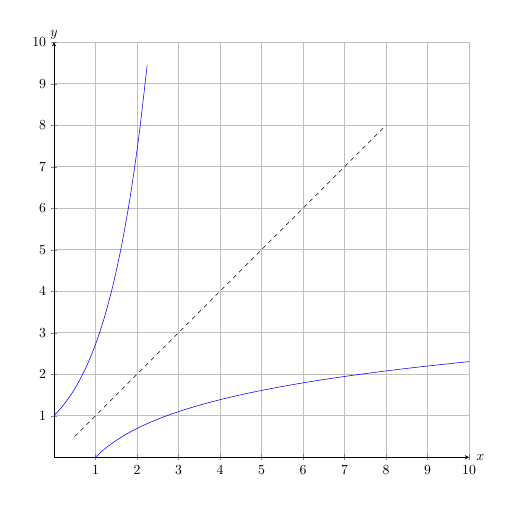
\begin{tikzpicture}[scale=.5]
		\begin{axis}[
			xmin=0,xmax=10,
			restrict y to domain=0:10,
			ymin=0,ymax=10,
			grid=both,width=\textwidth,height=\textwidth,
			axis lines=middle,
			xlabel={\(x\)},
			ylabel={\(y\)},
			enlarge x limits=0.1,
			enlarge y limits=0.1,
			axis lines = middle,
			x label style={at={(ticklabel* cs:1.00)}, inner sep=5pt, anchor=west},
			y label style={at={(ticklabel* cs:1.00)}, inner sep=2pt, anchor=south},
		]
			\addplot[color=blue,samples=50,smooth,domain=0:10]{exp(x)};
			\addplot[color=blue,samples=50,smooth,domain=1:10]{ln(x)};
			\addplot[color=black,dashed,domain=.5:8]{x};
		\end{axis}
	\end{tikzpicture}
	\caption{}\label{figure:函数.直接函数与反函数的图形的对称性}
\end{figure}

\begin{definition}
设函数\(y=f(u)\)的定义域为\(D_f\),
函数\(u=g(x)\)的定义域为\(D_g\),
且其值域\(R_g \subseteq D_f\),
则函数\[
	y = f[g(x)],
	\quad x \in D_g
\]
称为由函数\(u=g(x)\)与函数\(y=f(u)\)构成的\DefineConcept{复合函数},
它的定义域为\(D_g\),变量\(u\)称为\DefineConcept{中间变量}.

函数\(g\)与函数\(f\)构成的复合函数,
即按“先\(g\)后\(f\)”的次序复合的函数,
通常记为\(f \circ g\),即\[
	(f \circ g)(x) = f[g(x)].
\]
\end{definition}

\begin{example}
设函数\(f(x)\)的定义域为\((-l,l)\),
试证:在\((-l,l)\)上必存在偶函数\(g(x)\)和奇函数\(h(x)\),使得\[
	f(x) = g(x)+h(x).
\]
\begin{proof}
首先假设这样的\(g(x)\)、\(h(x)\)存在,即\[
	f(x) = g(x) + h(x),
\]\[
	g(-x) = g(x),
\]\[
	h(-x) = -h(x).
\]
于是有\[
	f(-x) = g(-x) + h(-x) = g(x) - h(x).
\]

由此可知,只需要取\[
	g(x) = \frac{1}{2} [f(x) + f(-x)],
\]\[
	h(x) = \frac{1}{2} [f(x) - f(-x)],
\]
即可满足题设要求.
\end{proof}
\end{example}
